\documentclass[a4paper]{article}

\usepackage[pdftex,
  hidelinks,
  pdfauthor={Dexter Chua},
  pdfsubject={Cambridge Maths Notes: Part IB - Statistics},
  pdftitle={Part IB - Statistics},
pdfkeywords={Cambridge Mathematics Maths Math IB Lent Statistics}]{hyperref}

\title{Part IB - Statistics}
\author{Lectured by D. Spiegelhalter}
\date{Lent 2015}

% Imports
\ifx \nextra \undefined
  \usepackage[pdftex,
    hidelinks,
    pdfauthor={Dexter Chua},
    pdfsubject={Cambridge Maths Notes: Part \npart\ - \ncourse},
    pdftitle={Part \npart\ - \ncourse},
  pdfkeywords={Cambridge Mathematics Maths Math \npart\ \nterm\ \nyear\ \ncourse}]{hyperref}
  \title{Part \npart\ - \ncourse}
\else
  \usepackage[pdftex,
    hidelinks,
    pdfauthor={Dexter Chua},
    pdfsubject={Cambridge Maths Notes: Part \npart\ - \ncourse\ (\nextra)},
    pdftitle={Part \npart\ - \ncourse\ (\nextra)},
  pdfkeywords={Cambridge Mathematics Maths Math \npart\ \nterm\ \nyear\ \ncourse\ \nextra}]{hyperref}

  \title{Part \npart\ - \ncourse \\ {\Large \nextra}}
\fi

\author{Lectured by \nlecturer \\\small Notes taken by Dexter Chua}
\date{\nterm\ \nyear}

\usepackage{alltt}
\usepackage{amsfonts}
\usepackage{amsmath}
\usepackage{amssymb}
\usepackage{amsthm}
\usepackage{booktabs}
\usepackage{caption}
\usepackage{enumitem}
\usepackage{fancyhdr}
\usepackage{graphicx}
\usepackage{mathtools}
\usepackage{microtype}
\usepackage{multirow}
\usepackage{pdflscape}
\usepackage{pgfplots}
\usepackage{siunitx}
\usepackage{tabularx}
\usepackage{tikz}
\usepackage{tkz-euclide}
\usepackage[normalem]{ulem}
\usepackage[all]{xy}

\pgfplotsset{compat=1.12}

\pagestyle{fancyplain}
\lhead{\emph{\nouppercase{\leftmark}}}
\ifx \nextra \undefined
  \rhead{
    \ifnum\thepage=1
    \else
      \npart\ \ncourse
    \fi}
\else
  \rhead{
    \ifnum\thepage=1
    \else
      \npart\ \ncourse\ (\nextra)
    \fi}
\fi
\usetikzlibrary{arrows}
\usetikzlibrary{decorations.markings}
\usetikzlibrary{decorations.pathmorphing}
\usetikzlibrary{positioning}
\usetikzlibrary{fadings}
\usetikzlibrary{intersections}
\usetikzlibrary{cd}

\newcommand*{\Cdot}{\raisebox{-0.25ex}{\scalebox{1.5}{$\cdot$}}}
\newcommand {\pd}[2][ ]{
  \ifx #1 { }
    \frac{\partial}{\partial #2}
  \else
    \frac{\partial^{#1}}{\partial #2^{#1}}
  \fi
}

% Theorems
\theoremstyle{definition}
\newtheorem*{aim}{Aim}
\newtheorem*{axiom}{Axiom}
\newtheorem*{claim}{Claim}
\newtheorem*{cor}{Corollary}
\newtheorem*{defi}{Definition}
\newtheorem*{eg}{Example}
\newtheorem*{fact}{Fact}
\newtheorem*{law}{Law}
\newtheorem*{lemma}{Lemma}
\newtheorem*{notation}{Notation}
\newtheorem*{prop}{Proposition}
\newtheorem*{thm}{Theorem}

\renewcommand{\labelitemi}{--}
\renewcommand{\labelitemii}{$\circ$}
\renewcommand{\labelenumi}{(\roman{*})}

\let\stdsection\section
\renewcommand\section{\newpage\stdsection}

% Strike through
\def\st{\bgroup \ULdepth=-.55ex \ULset}

% Maths symbols
\newcommand{\bra}{\langle}
\newcommand{\ket}{\rangle}

\newcommand{\N}{\mathbb{N}}
\newcommand{\Z}{\mathbb{Z}}
\newcommand{\Q}{\mathbb{Q}}
\renewcommand{\H}{\mathbb{H}}
\newcommand{\R}{\mathbb{R}}
\newcommand{\C}{\mathbb{C}}
\newcommand{\Prob}{\mathbb{P}}
\renewcommand{\P}{\mathbb{P}}
\newcommand{\E}{\mathbb{E}}
\newcommand{\F}{\mathbb{F}}
\newcommand{\cU}{\mathcal{U}}
\newcommand{\RP}{\mathbb{RP}}
\newcommand{\CP}{\mathbb{CP}}

\newcommand{\ph}{\,\cdot\,}

\DeclareMathOperator{\sech}{sech}
\DeclareMathOperator{\cosech}{cosech}
\DeclareMathOperator{\cosec}{cosec}

\DeclareMathOperator{\covol}{covol}
\DeclareMathOperator{\vol}{vol}

\let\Im\relax
\let\Re\relax
\DeclareMathOperator{\Im}{Im}
\DeclareMathOperator{\Re}{Re}
\DeclareMathOperator{\im}{im}
\DeclareMathOperator{\image}{image}
\DeclareMathOperator{\Ann}{Ann}

\DeclareMathOperator*{\res}{res}
\DeclareMathOperator{\Res}{Res}
\DeclareMathOperator{\Ind}{Ind}

\DeclareMathOperator{\tr}{tr}
\DeclareMathOperator{\diag}{diag}
\DeclareMathOperator{\rank}{rank}
\DeclareMathOperator{\card}{card}
\DeclareMathOperator{\spn}{span}
\DeclareMathOperator{\adj}{adj}

\DeclareMathOperator{\erf}{erf}
\DeclareMathOperator{\erfc}{erfc}

\DeclareMathOperator{\ord}{ord}
\DeclareMathOperator{\Sym}{Sym}

\DeclareMathOperator{\sgn}{sgn}
\DeclareMathOperator{\orb}{orb}
\DeclareMathOperator{\stab}{stab}
\DeclareMathOperator{\ccl}{ccl}

\DeclareMathOperator{\lcm}{lcm}
\DeclareMathOperator{\hcf}{hcf}

\DeclareMathOperator{\Int}{Int}
\DeclareMathOperator{\id}{id}

\DeclareMathOperator{\betaD}{beta}
\DeclareMathOperator{\gammaD}{gamma}
\DeclareMathOperator{\Poisson}{Poisson}
\DeclareMathOperator{\binomial}{binomial}
\DeclareMathOperator{\multinomial}{multinomial}
\DeclareMathOperator{\Bernoulli}{Bernoulli}
\DeclareMathOperator{\like}{like}

\DeclareMathOperator{\var}{var}
\DeclareMathOperator{\cov}{cov}
\DeclareMathOperator{\bias}{bias}
\DeclareMathOperator{\mse}{mse}
\DeclareMathOperator{\corr}{corr}

\DeclareMathOperator{\otp}{otp}
\DeclareMathOperator{\dom}{dom}

\DeclareMathOperator{\Root}{Root}
\DeclareMathOperator{\supp}{supp}
\DeclareMathOperator{\rel}{rel}
\DeclareMathOperator{\Hom}{Hom}
\DeclareMathOperator{\Aut}{Aut}
\DeclareMathOperator{\Gal}{Gal}
\DeclareMathOperator{\Mat}{Mat}
\DeclareMathOperator{\End}{End}
\DeclareMathOperator{\Char}{char}
\DeclareMathOperator{\ev}{ev}
\DeclareMathOperator{\St}{St}
\DeclareMathOperator{\Lk}{Lk}
\DeclareMathOperator{\disc}{disc}
\DeclareMathOperator{\Isom}{Isom}
\DeclareMathOperator{\length}{length}
\DeclareMathOperator{\energy}{energy}
\DeclareMathOperator{\area}{area}
\DeclareMathOperator{\Syl}{Syl}
\DeclareMathOperator{\cl}{cl}
\DeclareMathOperator{\fix}{fix}

\newcommand{\GL}{\mathrm{GL}}
\newcommand{\SL}{\mathrm{SL}}
\newcommand{\PGL}{\mathrm{PGL}}
\newcommand{\PSL}{\mathrm{PSL}}
\newcommand{\PSU}{\mathrm{PSU}}
\newcommand{\Or}{\mathrm{O}}
\newcommand{\SO}{\mathrm{SO}}
\newcommand{\U}{\mathrm{U}}
\newcommand{\SU}{\mathrm{SU}}

\renewcommand{\d}{\mathrm{d}}
\newcommand{\D}{\mathrm{D}}

\tikzset{->/.style = {decoration={markings,
                                  mark=at position 1 with {\arrow[scale=2]{latex'}}},
                      postaction={decorate}}}
\tikzset{<-/.style = {decoration={markings,
                                  mark=at position 0 with {\arrowreversed[scale=2]{latex'}}},
                      postaction={decorate}}}
\tikzset{<->/.style = {decoration={markings,
                                   mark=at position 0 with {\arrowreversed[scale=2]{latex'}},
                                   mark=at position 1 with {\arrow[scale=2]{latex'}}},
                       postaction={decorate}}}
\tikzset{->-/.style = {decoration={markings,
                                   mark=at position #1 with {\arrow[scale=2]{latex'}}},
                       postaction={decorate}}}
\tikzset{-<-/.style = {decoration={markings,
                                   mark=at position #1 with {\arrowreversed[scale=2]{latex'}}},
                       postaction={decorate}}}

\tikzset{circ/.style = {fill, circle, inner sep = 0, minimum size = 3}}
\tikzset{mstate/.style={circle, draw, blue, text=black, minimum width=0.7cm}}

\definecolor{mblue}{rgb}{0.2, 0.3, 0.8}
\definecolor{morange}{rgb}{1, 0.5, 0}
\definecolor{mgreen}{rgb}{0.1, 0.4, 0.2}
\definecolor{mred}{rgb}{0.5, 0, 0}

\def\drawcirculararc(#1,#2)(#3,#4)(#5,#6){%
    \pgfmathsetmacro\cA{(#1*#1+#2*#2-#3*#3-#4*#4)/2}%
    \pgfmathsetmacro\cB{(#1*#1+#2*#2-#5*#5-#6*#6)/2}%
    \pgfmathsetmacro\cy{(\cB*(#1-#3)-\cA*(#1-#5))/%
                        ((#2-#6)*(#1-#3)-(#2-#4)*(#1-#5))}%
    \pgfmathsetmacro\cx{(\cA-\cy*(#2-#4))/(#1-#3)}%
    \pgfmathsetmacro\cr{sqrt((#1-\cx)*(#1-\cx)+(#2-\cy)*(#2-\cy))}%
    \pgfmathsetmacro\cA{atan2(#2-\cy,#1-\cx)}%
    \pgfmathsetmacro\cB{atan2(#6-\cy,#5-\cx)}%
    \pgfmathparse{\cB<\cA}%
    \ifnum\pgfmathresult=1
        \pgfmathsetmacro\cB{\cB+360}%
    \fi
    \draw (#1,#2) arc (\cA:\cB:\cr);%
}
\newcommand\getCoord[3]{\newdimen{#1}\newdimen{#2}\pgfextractx{#1}{\pgfpointanchor{#3}{center}}\pgfextracty{#2}{\pgfpointanchor{#3}{center}}}

\def\Xint#1{\mathchoice
   {\XXint\displaystyle\textstyle{#1}}%
   {\XXint\textstyle\scriptstyle{#1}}%
   {\XXint\scriptstyle\scriptscriptstyle{#1}}%
   {\XXint\scriptscriptstyle\scriptscriptstyle{#1}}%
   \!\int}
\def\XXint#1#2#3{{\setbox0=\hbox{$#1{#2#3}{\int}$}
     \vcenter{\hbox{$#2#3$}}\kern-.5\wd0}}
\def\ddashint{\Xint=}
\def\dashint{\Xint-}


\begin{document}
\maketitle
{\small
\noindent\textbf{Estimation}\\
Review of distribution and density functions, parametric families. Examples: binomial, Poisson, gamma.  Sufficiency, minimal sufficiency, the Rao-Blackwell theorem. Maximum likelihood estimation. Confidence intervals. Use of prior distributions and Bayesian inference.\hspace*{\fill} [5]

\vspace{10pt}
\noindent\textbf{Hypothesis testing}\\
Simple examples of hypothesis testing, null and alternative hypothesis, critical region, size, power, type I and type II errors, Neyman-Pearson lemma. Significance level of outcome. Uniformly most powerful tests. Likelihood ratio, and use of generalised likelihood ratio to construct test statistics for composite hypotheses. Examples, including $t$-tests and $F$-tests. Relationship with confidence intervals. Goodness-of-fit tests and contingency tables.\hspace*{\fill} [4]

\vspace{10pt}
\noindent\textbf{Linear models}\\
Derivation and joint distribution of maximum likelihood estimators, least squares, Gauss-Markov theorem. Testing hypotheses, geometric interpretation. Examples, including simple linear regression and one-way analysis of variance. Use of software.\hspace*{\fill} [7]}

\tableofcontents

\section{Introduction and probability review}
*Lecturer apologizes for not turning up the previous lecture*
\begin{defi}[Statistics]
  \emph{Statistics} is a set of principle a nd procedures for gaining and processing quantitative evidence in order to help us make judgements and decisions.
\end{defi}
Note that we did not mention data. We don't necessarily need data for statistics (even though most often we do).

In this course, we focus on formal \emph{statistical inference}. In the process, we assume
\begin{itemize}
  \item we have data generated from some unknown probability model
  \item we aim to use the data to learn about certain properties of the underlying probability model
\end{itemize}
In particular, we perform parametric inference:

We assume a random variable $X$ takes values in $\mathcal{X}$. We assume its distribution belongs to a family of distribution (eg. Poisson) indexed by a scalar or vector parameter $\theta$, taking values in some parameter space $\Theta$. We call this a \emph{parametric family}.

For example, we can have $X\sim \text{Poisson}(\mu)$ and $\theta = \mu\in\Theta = (0, \infty)$.

We assume that we already which family it belongs to, and then try to find out $\theta$.

Suppose $X_1, X_2, \cdots, X_n$ are iid with the same distribution as $X$. Then $\mathbf{X} = (X_1, X_2, \cdots, X_n)$ is a simple random sample (ie. our data).

We use the observed $\mathbf{X} = \mathbf{x}$ to make inferences about $\theta$, such as
\begin{itemize}
  \item giving an estimate $\hat{\theta}(\mathbf{x})$ of the true value of $\theta$.
  \item Giving an interval estimate $(\hat{\theta}_1(\mathbf{x}), \hat{\theta}_2(\mathbf{x}))$ for $\theta$
  \item testing a hypothesis about $\theta$, eg. whether $\theta = 0$.
\end{itemize}
\section{Estimation, bias and mean squared error}
Suppose that $X_1, \cdots, X_n$ are iid, each with a probability density/mass function $f_X(x|\theta)$. We know $f_X$ but not $\theta$.

\begin{defi}[Statistic]
  A \emph{statistic} is an estimate of $\theta$. It is a function $T$ of a data. If $\mathbf{X} = \mathbf{x} = (x_1, \cdots, x_n)$, then our estimate is written as $\hat{\theta} = T(\mathbf{x})$. $T(\mathbf{X})$ is an \emph{estimator} of $\theta$.

  The distribution of $T = T(\mathbf{X})$ is its sampling distribution.

  Note that capital $\mathbf{X}$ denotes a random variable and $\mathbf{x}$ is an observed value. So $T(\mathbf{X})$ is a random variable and $T(\mathbf{x})$ is a particular value.
\end{defi}

\begin{eg}
  Let $X_1, \cdots, X_n$ is an iid $N(\mu, 1)$. A possible estimator for $\mu$ is
  \[
    T(\mathbf{X}) = \frac{1}{n}\sum X_i.
  \]
  The for any particular observed sample $\mathbf{x}$, our estimate is
  \[
    T(\mathbf{x}) = \frac{1}{n}\sum x_i.
  \]
  Recall that in general, if $X_i \sim N(\mu_i, \sigma_i^2)$, then $\sum X_i \sim N(\sum \mu_i, \sum \sigma_i^2)$, which can be proved by moment-generating functions.
  
  So we have $T(\mathbf{X})\sim N(\mu, 1/n)$. Note that by the Central Limit Theorem, even if $X_1$ were not normal, we still have $T(\mathbf{X})\sim N(\mu, 1/n)$ for large values of $n$.
\end{eg}

\begin{defi}[Bias]
  Let $\hat{\theta} = T(\mathbf{X})$ be an estimator of $\theta$. The \emph{bias} of $\hat{\theta}$ is the difference between its expected value and true value.
  \[
    \bias(\hat{\theta}) = \E_\theta(\hat{\theta}) - \theta.
  \]
  Note that the subscript $_\theta$ does not represent the random variable, but the thing we want to estimate. This is inconsistent with the use for, say the pmf.

  An estimator is \emph{unbiased} if it has no bias, ie. $\E_\theta(\hat{\theta}) = \theta$.
\end{defi}
To find out $\E_\theta (T)$, we can either find the distribution of $T$ and find its expected value, or evaluate $T$ as a function of $\mathbf{X}$ directly, and find its expected value. 

\begin{eg}
  In the above example, $\E_\mu(T) =\mu$. So $T$ is unbiased for $\mu$. 
\end{eg}
\subsection{Mean squared error}
In general, we prefer estimators whose sampling distributions ``cluster more closely'' around the true value of $\theta$.
\begin{defi}[Mean squared error]
  The \emph{mean squared error} of an estimator $\hat{\theta}$ is $\E_\theta[(\hat{\theta} - \theta)^2]$.

  Sometimes, we use the \emph{root mean squared error}, that is the square root of the above.
\end{defi}
For an unbiased estimator, the mean squared error is just the variance. In general,
\begin{align*}
  \E_\theta[(\hat{\theta} - \theta)^2] &= \E_\theta[(\hat{\theta} - E_\theta(\hat{\theta}) + \E_\theta(\hat{\theta}) - \theta)^2]\\
  &= \E_\theta[(\hat{\theta} - E_\theta(\hat{\theta}))^2] + \E_\theta(\hat{\theta}) - \theta]^2 + 2[\E_\theta(\hat{\theta}) - \theta]\E_\theta[\hat{\theta} - \E_\theta(\hat{\theta})]\\
  &= \var(\hat{\theta}) + \bias^2(\hat{\theta}).
\end{align*}
Sometimes it can be preferable to have a biased estimator with a low variance - sometimes know as the ``bias-variance trade-off''.

For example, suppose $X\sim \binomial(n, \theta)$. The standard estimator is $T_U = \mathbf{X}/n$, which is unbiased. $T_U$ has variance
\[
  \var_\theta(T_U) = \var_\theta(\mathbf{X})/n^2 = \theta(1 - \theta)/n.
\]
Consider an alternative estimator 
\[
  T_B = \frac{X + 1}{n + 2} = w\frac{X}{n} + (1 - w)\frac{1}{2},
\]
where $w = n/(n + 2)$. This can be interpreted to be a weighted average (by the sample size) of the sample mean and $1/2$. We have
\[
  \E_\theta(T_B) - \theta = \frac{n\theta + 1}{n + 2} - \theta = (1 - w)\left(\frac{1}{2} - \theta\right),
\]
and is biased. However,
\[
  \var_\theta(T_B) = \frac{\var_\theta(\mathbf{X})}{(n + 2)^2} = w^2\theta(1 - \theta)/n
\]
Now
\[
  \mse (T_U) = \var_\theta(T_U) + \bias^2(T_U) = \theta(1 - \theta)/n.
\]
and
\[
  \mse (T_B) = \var_\theta(T_B) + \bias^2(T_B) = w^2\frac{\theta(1 - \theta)}{n} + (1 - w)^2\left(\frac{1}{2} - \theta\right)^2
\]
We can plot the mean squared error for possible values of $\theta$. Here we plot the case where $n = 10$.
\begin{center}
  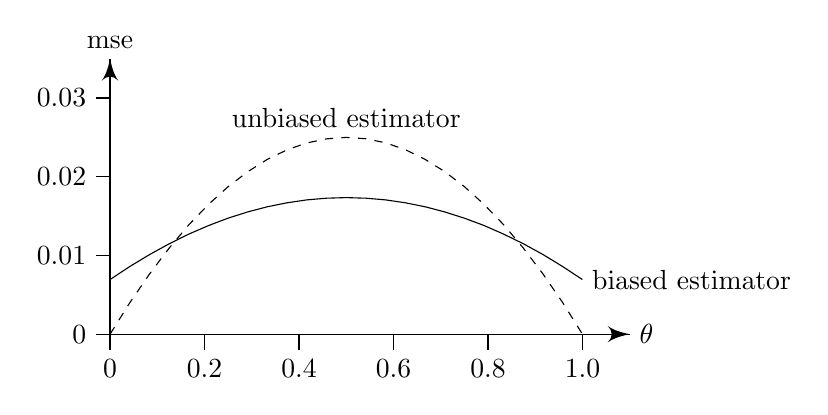
\begin{tikzpicture}[xscale=6,yscale=100]
    \draw [dashed, domain=0:1] plot (\x, {\x * (1 - \x) / 10});
    \node [above] at (0.5, 0.025) {unbiased estimator};
    \draw [domain=0:1] plot (\x, {25 * \x * (1 - \x) / 360 + (1 - 5/6)*(1 - 5/6)*(0.5 - \x)*(0.5 - \x)}) node [right] {biased estimator};
    \draw [->] (0, 0) -- (1.1, 0) node [right] {$\theta$};
    \draw [->] (0, 0) -- (0, 0.035) node [above] {mse};
    \foreach \x in {0, 0.2, 0.4, 0.6, 0.8, 1.0} {
      \draw (\x, 0) -- (\x, -0.002) node [below] {\x};
    }
    \foreach \y in {0, 0.01, 0.02, 0.03} {
      \draw (0, \y) -- (-.03, \y) node [left] {\y};
    }
  \end{tikzpicture}
\end{center}
We see that this biased estimator has smaller MSE unless $\theta$ has extreme values.

Also, suppose $X\sim \Poisson(\lambda)$, and for some reason, you want to estimate $\theta = [P(\mathbf{X} = 0)]^2 = e^{-2\lambda}$. Then any estimator $T(\mathbf{X})$ must satisfy $\E_\theta(T(\mathbf{X})) = \theta$, or equivalently,
\[
  E_\lambda(T(\mathbf{X})) = e^{-\lambda}\sum_{x = 0}^\infty T(x) \frac{\lambda^x}{x!} = e^{-2\lambda}.
\]
Then the only function $T$ that can satisfy this equation is $T(X) = (-1)^X$.

Then the only unbiased estimator estimate $e^{-2\lambda}$ to be $1$ if $X$ is even, -1 if $X$ is odd. CLEARLY crazy. 
\section{Sufficiency}
``Sufficiency'' is the question ``Is there a statistic $T(\mathbf{X})$ that in some sense contains all the information about $\theta$ that is in the sample?'' This is important in ``big data'' in which we have to store a large number of data.

\begin{eg}
  Let $X_1, \cdots X_n$ be iid $\Bernoulli(\theta)$, so that $\P(X_i = 1) = 1 - \P(X_i = 0) = \theta$ for some $0 < \theta < 1$. So
  \[
    f_{\mathbf{X}} (\mathbf{x}|\theta) = \prod_{i = 1}^n \theta^{x_i}(1 - \theta)^{1 - x_i} = \theta^{\sum x_i}(1 - \theta)^{n - \sum x_i}.
  \]
  This depends on the data only through $T(\mathbf{X}) = \sum x_i$, the total number of ones. Note that $T(\mathbf{X})\sim \binomial(n, \theta)$.

  If $T(\mathbf{x}) = t$, then
  \[
    f_{\mathbf{X}|T = t} = \frac{\P_\theta(\mathbf{X} = \mathbf{x}, T = t)}{\P_\theta T = t} = \frac{\P_\theta(\mathbf{X} = \mathbf{x})}{T = t}.
  \]
  Where the last equality comes because since if $\mathbf{X} = \mathbf{x}$, then $T$ must be equal to $t$. This is equal to
  \[
    \frac{\theta^{\sum x_i}(1 - \theta)^{n - \sum x_i}}{\binom{n}{t}\theta^t (1 - \theta)^{n - t}} = \binom{n}{t}^{-1}.
  \]
  So we know that the conditional distribution of $\mathbf{X}$ given $T = t$ does not depend on $\theta$. So if we know $T$, then additional knowledge of $\mathbf{x}$ does not give more information about $\theta$.
\end{eg}

\begin{defi}[Sufficient statistic]
  A statistic $T$ is \emph{sufficient} for $\theta$ if the conditional distribution of $\mathbf{X}$ given $T$ does not depend on $\theta$.
\end{defi}

In practice, we find them as follows:
\begin{thm}[The factorization criterion]
  $T$ is sufficient for $\theta$ iff $f_{\mathbf{X}}(\mathbf{x} |\theta) = g(T(\mathbf{x}), \theta)h(\mathbf{x})$ for some functions $g$ and $h$.
\end{thm}

\begin{proof}
  (discrete case only)

  Suppose $f_\mathbf{X}(\mathbf{x}|\theta) = g(T(\mathbf{x}, \theta)h(\mathbf{x})$. If $T(\mathbf{x}) = t$, then
  \begin{align*}
    f_{\mathbf{X}|T = t}(\mathbf{x}|T = t) &= \frac{\P_\theta(\mathbf{X} = \mathbf{x}, T(\mathbf{X}) = t)}{\P_\theta (T = t)}\\
    &= \frac{g(T(\mathbf{x}), \theta)h(\mathbf{x})}{\sum_{\{x:T(\mathbf{x}) = t\}}g(T(\mathbf{x}), \theta)h(\mathbf{x})}\\
    &=\frac{g(t, \theta)h(\mathbf{x})}{g(t, \theta)\sum h(\mathbf{x})}\\
    &= \frac{h(\mathbf{x})}{\sum h(\mathbf{x})}
  \end{align*}
  which doesn't depend on $\theta$. So $T$ is sufficient.

  Now suppose $T$ is sufficient so that the conditional distribution of $\mathbf{X}|T = t$ does not depend on $\theta$. If $T(\mathbf{x}) = t$, then
  \[
    \P_\theta(\mathbf{X} = \mathbf{x}) = \P_\theta(\mathbf{X} = \mathbf{x}, T=t') = \P_\theta(\mathbf{X} = \mathbf{x}|T = t)\P_\theta (T = t).
  \]

  The first factor does not depend on $\theta$ by assumption; call it $h(\mathbf{x})$. Let the second factor be $g(t, \theta)$, and so we have the required factorisation.
\end{proof}

\begin{eg}
  Continuing the above example,
  \[
    f_\mathbf{X}(\mathbf{x}|\theta) = \theta^{\sum x_i}(1 - \theta)^{n - \sum x_i}.
  \]
  Take $g(t, \theta) = \theta^t(1 - \theta)^{n - t}$ and $h(\mathbf{x}) = 1$ to see that $T(\mathbf{X}) = \sum X_i$ is sufficient for $\theta$.
\end{eg}

\begin{eg}
  Let $X_1, \cdots, X_n$ be iid $U[0, \theta]$. Write $1_{[A]}$ for the indicator function of $A$. We have
  \[
    f_\mathbf{X}(\mathbf{x}|\theta) = \prod_{i = 1}^n \frac{1}{\theta}1_{[0 \leq x_i\leq \theta]} = \frac{1}{\theta^n}1_{[\max_i x_i \leq \theta]}1_{[\min_i x_i\geq 0]}.
  \]
  So $T = \max_i x_i$ is sufficient.
\end{eg}

Note that sufficient statistics are not unique. If $T$ is sufficient for $\theta$, then so is any 1-1 function of $T$. $\mathbf{X}$ is always sufficient for $\theta$ as well, but it is not of much use.


The sample space $\mathcal{X}^n$ is partitioned by $T$ into sets $\{\mathbf{x}\in \mathcal{X}: t(\mathbf{X}) = t\}$. If $T$ is sufficient, then this data reduction does not lose any information on $\theta$. We seek a sufficient statistic that achieves the maximum-possible reduction.

\begin{defi}[Minimal sufficiency]
  A sufficient statistic $T(\mathbf{x})$ is minimal if it is a function of every other sufficient statistic, ie. if $T'(\mathbf{X})$ is also sufficient, then $T'(\mathbf{X}) = T'(\mathbf{Y}) \Rightarrow  T(\mathbf{X}) = T(\mathbf{Y})$. ie. it has the coarsest partitions.
\end{defi}

We can find them using the following theorem:
\begin{thm}
  Suppose $T = T(\mathbf{X})$ is a statistic such that $f_\mathbf{X}(\mathbf{x}; \theta)/f_\mathbf{X}(\mathbf{y}; \theta)$ is a constant as a function of $\theta$ if and only if $T(\mathbf{x}) = T(\mathbf{y})$. Then $T$ is minimal sufficient for $\theta$.
\end{thm}

\begin{eg}
  Suppose $X_1, \cdots, X_n$ are iid $N(\mu, \sigma^2)$. Then
  \begin{align*}
    \frac{f_\mathbf{X}(\mathbf{x}|\mu, \sigma^2)}{f_\mathbf{X}(\mathbf{y}|\mu, \sigma^2)} &= \frac{(2\pi\sigma^2)^{-n/2}\exp\left\{-\frac{1}{2\sigma^2}\sum_i(x_i - \mu)^2\right\}}{(2\pi\sigma^2)^{-n/2}\exp\left\{-\frac{1}{2\sigma^2}\sum_i(y_i - \mu)^2\right\}}\\
    &=\exp\left\{-\frac{1}{2\sigma^2}\left(\sum_i x_i^2 - \sum_i y_i^2\right) + \frac{\mu}{\sigma^2}\left(\sum_{i}x_i - \sum_i y_i\right)\right\}.
  \end{align*}
  This is a constant function of $(\mu, \sigma^2)$ iff  $\sum_i x_i^2 = \sum_i y_i^2$ and $\sum_i x_i = \sum_i y_i$. So $T(\mathbf{X}) = (\sum_i X_i^2, \sum_i X_i)$ is minimal sufficient for $(\mu, \sigma^2)$.
\end{eg}
\note If the range of $\mathbf{X}$ depends on $\theta$, then ``$f_\mathbf{X}(\mathbf{x}; \theta)/f_\mathbf{X}(\mathbf{y};\theta)$ is constant in $\theta$'' means ``$f_\mathbf{X}(\mathbf{x}; \theta = c(\mathbf{x}, \mathbf{y})f_\mathbf{X}(\mathbf{y}; \theta)$''

\begin{thm}[Rao-Blackwell Theorem]
  Let $T$ be a sufficient statistic for $\theta$ and let $\tilde{\theta}$ be an estimator for $\theta$ with $\E(\tilde{\theta}^2) < \infty$ for all $\theta$. Let $\hat{\theta} = \E[\hat{\theta}|T]$. Then for all $\theta$,
  \[
    \E[(\hat{\theta} - \theta)^2] \leq \E[(\tilde{\theta} - \theta)^2].
  \]
  The inequality is strict unless $\tilde{\theta}$ is a function of $T$.
\end{thm}

\begin{proof}
  By the conditional expectation formula, we have $\E(\hat{\theta}) = \E[\E(\tilde{\theta}|T)] = E(\tilde{\theta})$. So they have the same bias.

  By the conditional variance formula,
  \[
    \var(\tilde{\theta}) = \E[\var (\tilde{\theta}|T)] + \var [\E(\tilde{\theta}|T)] = \E[\var(\tilde{\theta}|T)] + \var(\hat{\theta}).
  \]
  Hence $\var(\tilde{\theta}) \geq \var (\hat{\theta})$. So $\mse(\tilde{\theta} \geq \mse\hat{\theta})$, with equality only if $\var(\tilde{\theta}|T) = 0$.
\end{proof}
\note
\begin{enumerate}
  \item Since $T$ is sufficient for $\theta$, the conditional distribution of $\mathbf{X}$ given $T = t$ does not depend on $\theta$. Hence $\hat{\theta} = \E[\tilde{\theta}(\mathbf{X})|T]$ does not depend on $\theta$, and so is a genuine estimator.
  \item The theorem says that given any estimator, we can find one that is a function of a sufficient statistic that is at least as good in terms of mean squared error of estimation.
  \item If $\tilde{\theta}$ is unbiased, then so is $\hat{\theta}$.
  \item If $\tilde{\theta}$ is already a function of $T$, then $\hat{\theta} = \tilde{\theta}$.
\end{enumerate}

\begin{eg}
  Suppose $X_1, \cdots, X_n$ are iid $\Poisson(\lambda)$, and let $\theta = e^{-\lambda}$ (ie. $\P(X_1 = 0)$. Then
  \[
    p_\mathbf{X}(\mathbf{x}|\lambda) =\frac{-e^{n\lambda}\lambda^{\sum x_i}}{\prod x_i!}.
  \]
  So
  \[
    p_\mathbf{X}(\mathbf{x}|\theta) = \frac{\theta^n(-\log \theta)^{\sum x_i}}{\prod x_i!}.
  \]
  We see that $T = \sum X_i$ is sufficient for $\theta$, and $\sum X_i \sim \Poisson (n\lambda)$.

  We use an easy estimator $\theta$ is $\tilde{\theta} = 1_{X_1 = 0}$, which is unbiased. (ie. if we observe nothing in the first observation period, we assume the event is impossible) Then
  \begin{align*}
    \E[\tilde{\theta}| T = t] &= \P\left(X_1 = 0|\sum_1^n X_i = t\right)\\
    &= \frac{\P(X_1 = 0)\P(\sum_2^n X_i = t)}{\P(\sum_1^n X_i = t)}\\
    &= \left(\frac{n - 1}{n}\right)^t.
  \end{align*}
  So $\hat{\theta} = (1 - 1/n)^{\sum x_i}$. This approximately $(1 - 1/n)^{n\bar{X}} \approx e^{-\bar X} = e^{-\hat{\lambda}}$, which makes sense.
\end{eg}

\begin{eg}
  Let $X_1, \cdots X_n$ be iid $U[0, \theta]$, and suppose that we want to estimate $\theta$. We have shown above that $T = \max X_i$ is sufficient for $\theta$. Let $\hat{\theta} = 2X_1$, and unbiased estimator. Then
  \begin{align*}
    \E[\tilde{\theta}|T = t] &= 2\E[X_1|\max X_i = t]\\
    &= 2(E[X_1|\max X_i = t, X_1 = \max X_i]\P(X_1 = \max X_i)\\
    &+ \E[X_1|\max X_i = t, X_1 \not= \max X_i] \P(X_1 \not= \max X_i))\\
    &= 2\left(t\times \frac{1}{n} + \frac{t}{2}\frac{n - 1}{n}\right)\\
    &= \frac{n + 1}{n}t.
  \end{align*}
  So $\hat{\theta} = \frac{n + 1}{n}\max X_i$.
\end{eg}

\section{Likelihood}
Maximum likelihood estimation is one of the most important and widely used methods for finding estimations. Let $X_1, \cdots , X_n$ be random variables with joint pdf/pmg $f_\mathbf{X}(\mathbf{x}|\theta)$. We observe $\mathbf{X} = \mathbf{x}$.

\begin{defi}[Likelihood]
  The \emph{likelihood} of $\theta$ is $\like(\theta) = f_\mathbf{X}(\mathbf{x} | \theta)$, regarded as a function of $\theta$. The \emph{maximum likelihood estimator} (mle) of $\theta$ is the value of $\theta$ that maximizes $\like (\theta)$.
\end{defi}
It is often easier to maximize the \emph{log-likelihood}.

If $X_1, \cdots, X_n$ are iid, each with pdf/pmf $f_X(x|\theta)$, then
\begin{align*}
  \like(\theta) &= \prod_{i = 1}^n f_X(x_i|\theta)\\
  \log\like (\theta) &= \sum_{i = 1}^n \log f_X(x_i|\theta).
\end{align*}

\begin{eg}
  Let $X_1, \cdots, X_n$ be iid $\Bernoulli(p)$. Then
  \[
    l(p) =\log\like(p) = \left(\sum x_i\right)\log p + \left(n - \sum x_i\right)\log(1 - p).
  \]
  Thus
  \[
    \frac{\d l}{\d p} = \frac{\sum x_i}{p} - \frac{n - \sum x_i}{1 - p}.
  \]
  This is zero when $p = \sum x_i /n$, and this is the maximum likelihood estimator. (and is unbiased)
\end{eg}

\begin{eg}
  Let $X_1, \cdots, X_n$ be iid $N(\mu, \sigma^2)$, $\theta = (\mu, \sigma^2)$. Then
  \[
    l(\mu, \sigma^2) = \log\like(\mu, \sigma^2) = -\frac{n}{2}\log (2\pi) - \frac{n}{2}\log (\sigma^2) - \frac{1}{2\sigma^2}\sum (x_i - \mu)^2.
  \]
  This is maximized when
  \[
    \frac{\partial l}{\partial\mu} = \frac{\partial l}{\partial \sigma^2} = 0.
  \]
  We have
  \[
    \frac{\partial l}{\partial \mu} = -\frac{1}{\sigma^2}\sum (x_i - \mu), \quad \frac{\partial l}{\sigma^2} = -\frac{n}{2\sigma^2} + \frac{1}{2\sigma^4}\sum (x_i - \mu)^2.
  \]
  So the solution, hence maximum likelihood estimator is $(\hat{\mu}, \hat{\sigma}^2) = (\bar x, S_{xx}/n)$, where $\bar{x} = \frac{1}{n}\sum x_i$ and $S_{xx} = \sum(x_i - \bar{x})^2$.

  We shall see later that $S_{XX}/s^2 = \frac{n\hat{\sigma}^2}{\sigma^2}\sim \chi_{n - 1}^2$, and so $\E(\hat{\sigma}^2) = \frac{(n - 1)\sigma^2}{n}$, ie. $\hat{\sigma}^2$ is biased.
\end{eg}

\begin{eg}
  Let $X_1, \cdots X_n$ be iid $U(0, \theta)$. This is the ``German tank problem'': suppose the American army discovers some German tanks that are sequentially numbered, i.e. the first tank is numbered 1, the second is numbered 2, etc. Then if $\theta$ tanks are produced, then the probability distribution of the tank number is $U(0, \theta)$. Suppose we have discovered $n$ tanks whose numbers are $x_1, x_2, \cdots, x_n$, and we want to estimate $\theta$, the total number of tanks produced. We want to find the maximum likelihood estimator.
  
  Then
  \[
    \like(\theta) = \frac{1}{\theta^n}1_{[\max x_i \leq \theta]}1_{[\min x_i\geq 0]}.
  \]
  So for $\theta\geq \max _i$, $\like (\theta) = 1/\theta^n$ and is decreasing as $\theta$ increases, while for $\theta < \max x_i$, $\like (\theta) = 0$. Hence the value $\hat{\theta} = \max x_i$ maximizes the likelihood.

  Is $\hat{\theta}$ unbiased? First we need to find the distribution of $\hat{\theta}$. For $0 \leq t \leq \theta$, the distribution function of $\hat{\theta}$ is
  \[
    F_{\hat{\theta}}(t) = P(\hat{\theta} \leq t) = \P(X_i \leq t, \text{all }i) = (\P(X_i \leq t))^n = \left(\frac{t}{\theta}\right)^n,
  \]
  Differentiating with respect to $T$, we find the $pdf f_{\hat{\theta}} = \frac{nt^{n - 1}}{\theta^n}$. Hence
  \[
    \E(\hat{\theta}) = \int_0^\theta t\frac{nt^{n - 1}}{\theta^n} \;\d t = \frac{n\theta}{n + 1}.
  \]
  So $\hat{\theta}$ is biased, but asymptotically unbiased.
\end{eg}

\note
\begin{enumerate}
  \item if $T$ is sufficient for $\theta$, then the likelihood is $g(T(\mathbf{x}), \theta)h(\mathbf{x})$, which depends on $\theta$ through $T(\mathbf{x})$. To maximise this as a function of $\theta$, we only need to maximize $g$, and so the mle $\hat{\theta}$ is a function of the sufficient statistic.
  \item If $\phi = h(\theta)$ with $h$ injective, then the mle of $\phi =h(\hat{\theta})$. If the mle of $\theta$ is $\hat{\theta}$, then the mle of $\theta^2$ is $\hat{\theta}^2$.
  \item Often there is no closed form for the mle, and we have to find $\hat{\theta}$ numerically.
\end{enumerate}

\begin{eg}
  Smarties come in $k$ equally frequent colours, but suppose we do not know $k$. Assume that we sample with replacement (although this is unhygienic).

  Our first Smarties are Red, Purple, Red, Yellow. Then
  \begin{align*}
  \like(k)&=\P_k(\text{1st is a new colour})\P_k(\text{2nd is a new colour})\\\
  & \P_k(\text{3rd matches 1st})\P_k(\text{4th is a new colour})\\
  &= 1\times \frac{k - 1}{k}\times \frac{1}{k}\times \frac{k - 2}{k}\\
  &= \frac{(k - 1)(k - 2)}{k^3}.
\end{align*}
The maximum likelihood is 5 (by trial and error), even though it is not much likelier than the others.
\end{eg}

\section{Confidence intervals}
\begin{defi}
  A $100\gamma\%$ ($0 < \gamma < 1$) \emph{confidence interval} (CO) for $\theta$ is a random interval $(A(\mathbf{X}), B(\mathbf{X}))$ such that $\P(A(\mathbf{X}) < \theta < B(\mathbf{X})) = \gamma$, no matter what the true value of $\theta$ may be.
\end{defi}

Notice that it is endpoints of the interval are random quantities, while $\theta$ is a fixed constant we want to find out.

We can interpret this in terms of repeat sampling. If we calculate $(A(\mathbf{x}), B(\mathbf{x}))$ for a large number of samples $\mathbf{x}$, then approximately $100\gamma\%$ of them will cover the true value of $\theta$.

IMPORTANT: having observed some data $\mathbf{x}$ and calculated $95\%$ confidence interval, we \emph{cannot} say that $\theta$ has 95\% chance of being within the interval.

\begin{eg}
  Suppose $X_1, \cdots, X_n$ are iid $N(\theta, 1)$. Find a $95\%$ confidence interval for $\theta$.

  We know $\bar X \sim N(\theta, \frac{1}{n}\sigma^2)$, so that $\sqrt{n}(\bar X - \theta)\sim N(0, 1)$.

  Let $z_1, z_2$ be such that $\phi(z_2) - \phi(z_1) = 0.95$, where $\phi$ is the standard normal distribution function.

  We have $\P[z_1 < \sqrt{n}(\bar X - \theta) < z_2] = 0.95$, which can be rearranged to give
  \[
    \P\left[\bar X - \frac{z_2}{\sqrt{n}} < \theta < \bar X - \frac{z_1}{\sqrt{n}}\right] = 0.95.
  \]
  so that
  \[
    \left(\bar X - \frac{z_2}{\sqrt{n}}, \bar X - \frac{z_1}{\sqrt{n}}\right).
  \]
  There are many possible choices for $z_1$ and $z_2$. Since $N(0, 1)$ density is symmetric, the shortest such interval is obtained by $z_2 = z_{0.025} = -z_1$. We can also choose other values such as $z_1 = -\infty$, $z_2 = 1.64$, but we usually choose symmetric end points.
\end{eg}
The above example illustrates a common procedure for finding confidence intervals:
\begin{itemize}
  \item Find a quantity $R(\mathbf{X}, \theta)$ such that the $\P_\theta$-distribution of $R(\mathbf{X}, \theta)$ does not depend on $\theta$. This is called a \emph{pivot}. In our example, $R(\mathbf{X}, \theta) = \sqrt{n}(\bar X - \theta)$.
  \item Write down a probability statement of the form $\P_\theta(c_1 < R(\mathbf{X}, \theta) < c_2) = \gamma$.
  \item Rearrange the inequalities inside $\P(\ldots)$ to find the interval.
\end{itemize}
\note
\begin{enumerate}
  \item Usually $C_1, c_2$ are percentage points from a know standardised distribution, often equitailed so that use, say, $2.5\%$ and $97.5\%$ points for a $95\%$ confidence interval. We could use, say $0\%$ and $95\%$, but the interval would generally be wider.
  \item We can have confidence intervals for vector parameters.
  \item IF $(A(\mathbf{x}, B(\mathbf{x}))$ is a $100\gamma\%$ confidence interval for $\theta$, and $T(\theta)$ is a monotone increasing function of $\theta$, then $(T(A(\mathbf{x})), T(B(\mathbf{x})))$ is a $100\gamma\%$ confidence interval for $T(\theta)$.
\end{enumerate}
\begin{eg}
  Suppose $X_1, \cdots, X_{50}$ are iid $N(0, \sigma^2)$. Find a $99\%$ confidence interval for $\sigma^2$.

  We know that $X_i/\sigma \sim N(0, 1)$. So $\displaystyle\frac{1}{\sigma^2}\sum_{i = 1}^{50}X_i^2 \sim \chi^2_{50}$.

  So $R(\mathbf{X}, \sigma^2) = \sum_{i = 1}^{50} X_2^2/\sigma^2$ is a pivot.

  Recall that $\chi_n^2(\alpha)$ is the upper $100\alpha\%$ point of $\chi_n^2$, ie.
  \[
    \P(\chi_n^2 \leq \chi_n^2(\alpha)) = 1 - \alpha.
  \]
  So we have $c_1 = \chi_{50}^2(0.995) = 27.99$ and $c_2 = \chi_{50}^2(0.005) = 79.49$.

  So
  \[
    \P \left(c_1 < \frac{\sum X_i^2}{\sigma^2} < c_2\right) = 0.99,
  \]
  and so
  \[
    \P\left(\frac{\sum X_i^2}{c_2} < \sigma^2 < \frac{\sum X_i^2}{c_1}\right) = 0.99.
  \]
  Furthermore, a $99\%$ confidence interval for $\sigma$ is $\left(\sqrt{\frac{\sum X_i^2}{c_2}}, \sqrt{\frac{\sum X_i^2}{c_1}}\right)$.
\end{eg}

\begin{eg}
  Suppose $X_1, \cdots, X_n$ are iid $\Bernoulli(p)$. Find an approximate confidence interval for $p$.

  The mle of $p$ is $\hat p = \sum X_i/n$.

  By the Central Limit theorem, $\hat{p}$ is approximately $N(p, p(1 - p)/n)$ for large $n$.

  So $\displaystyle \frac{\sqrt{n}(\hat{p} - p)}{\sqrt{p(1 - p)}}$ is approximately $N(0, 1)$ for large $n$. So we have
  \[
    \P\left(\hat p - z_{(1 - \gamma)/2}\sqrt{\frac{p(1 - p)}{n}} < p < \hat{p} + z_{(1 - \gamma)/2}\sqrt{\frac{p(1 - p)}{n}}\right)\approx \gamma.
  \]
  But $p$ is unknown! So we approximate it by $\hat{p}$ to get a confidence interval for $p$ when $n$ is large:
  \[
    \P\left(\hat p - z_{(1 - \gamma)/2}\sqrt{\frac{\hat p(1 - \hat p)}{n}} < p < \hat{p} + z_{(1 - \gamma)/2}\sqrt{\frac{\hat p(1 - \hat p)}{n}}\right)\approx \gamma.
  \]
\end{eg}

\begin{eg}
  Suppose an opinion poll says $20\%$ are going to vote $UKIP$, based on a random sample of $1,000$ people. What might the true proportion be?

  We assume we have an observation of $x = 200$ from a $\binomial(n, p)$ distribution with $n = 1,000$. Then $\hat p = x/n = 0.2$ is an unbiased estimate, also the mle. 
  Now $\var(X/n) = \frac{p(1 - p)}{n}\approx \frac{\hat p(1 - \hat p}{n} = 0.00016$.

  So a $85\%$ confidence interval is
  \[
    \left(\hat p - 1.96\sqrt{\frac{\hat p(1 - \hat p)}{n}}, \hat p + 1.96\sqrt{\frac{\hat p(1 - \hat p)}{n}}\right) = 0.20 \pm 1.96\times 0.013 = (0.175, 0.225),
  \]
  \note Since $p(1 - p)\leq 1/4$ for all $0 \leq p \leq 1$, then a conservative $95\%$ interval is $\hat p \pm 1.96\sqrt{1/4n} \approx \hat p \pm \sqrt{1/n}$. So whatever proportion is reported, it will be 'accurate' to $\pm 1/\sqrt{n}$. 
\end{eg}

\begin{eg}
  Suppose $X_1, X_2$ are iid from $U(\theta - 1/2, \theta + 1/2)$. What is a sensible $50\%$ confidence interval for $\theta$?

  Consider the probability of getting one observation on each side of $\theta$:
  \[
    \P_\theta(\min(X_1, X_2) \leq \theta \leq \max(X_1, X_2)) = \frac{1}{2}.
  \]
  So $(\min(X_1, X_2), \max (X_1, X_2))$ is a confidence interval for $\theta$.

  But suppose $|X_1 - X_2| \geq \frac{1}{2}$, e.g. $x_1 = 0.2, x_2 = 0.9$, then we \emph{know} that, in this particular case, $\theta$ \emph{must} lie in $(\min (X_1, X_2), \max(X_1, X_2))$. This means that we can get a much narrower $50\%$ confidence interval! So guaranteed sampling properties does not necessarily mean a sensible conclusion in all cases.
\end{eg}
\section{Bayesian estimation}
So far we have seen the \emph{frequentist} approach to a statistical inference, ie. inferential statements about $\theta$ are interpreted in terms of repeat sampling. For example, the confidence interval is what's the probability that the interval will contain $\theta$, not the probability that $\theta$ lies in the interval.

In contrast, the Bayesian approach treats $\theta$ as a random variable taking values in $\Theta$. The investigator's information and beliefs about the possible values of $\theta$ before any observation of data, are summarised by a \emph{prior distribution} $\pi(\theta)$. When $\mathbf{X} = \mathbf{x}$ are observed, the extra information about $\theta$ is combined with the prior to obtain the \emph{posterior distribution} $\pi(\theta|\mathbf{x})$ for $\theta$ given $\mathbf{X} = \mathbf{x}$.

There has been a long-running argument between the two approaches. Recently, things have settled down, and Bayesian methods are seen to be appropriate in huge numbers of application where one seeks to assess a probability about a ``state of the world''. For example, spam filters will assess the probability that a specific email is a spam, even though from a frequentist's point of view, this is nonsense, because the email either is or is not a spam, and it makes no sense to assign a probability to the email's being a spam.

In Bayesian inference, we usually have some \emph{prior} knowledge about the distribution of $\theta$ (eg. between $0$ and $1$). After collecting some data, we will find a \emph{posterior} distribution of $\theta$ given $\mathbf{X} = \mathbf{x}$.

\begin{defi}[Prior and posterior distribution]
  The \emph{prior distribution} of $\theta$ is the probability distribution of the value of $\theta$ before conducting the experiment. We usually write as $\pi(\theta)$. 

  The \emph{posterior distribution} of $\theta$ is the probability distribution of the value of $\theta$ given an outcome of the experiment $\mathbf{x}$. We write as $\pi(\theta|\mathbf{x})$.
\end{defi}
By Bayes' theorem, the distributions are related by
\[
  \pi(\theta|\mathbf{x}) = \frac{f_{\mathbf{X}}(\mathbf{x}|\theta)\pi(\theta)}{f_{\mathbf{X}}(\mathbf{x})}.
\]
Thus
\begin{align*}
  \pi(\theta|\mathbf{x}) &\propto f_{\mathbf{X}}(\mathbf{x}|\theta)\pi(\theta).\\
  \text{posterior} &\propto \text{likelihood}\times\text{prior}.
\end{align*}
where the constant of proportionality is chosen to make the total mass of the posterior distribution equal to one. Usually, we use this form, instead of attempting to calculate $f_\mathbf{X}(\mathbf{x})$.

In practice, we can recognise the family for $\pi(\theta|\mathbf{x})$. It should be clear that the data enter through the likelihood, so the inference is automatically based on any sufficient inference.

\begin{eg}
  Suppose I have $3$ coins in my pocket. One is $3:1$ in favour of tails, one is a fair coin, and one is $3:1$ in favour of heads.

  I randomly select one coin and flip it once, observing a head. What is the probability that I have chosen coin 3?

  Let $X = 1$ denote the event that I observe a head, $X = 0$ if a tail. Let $\theta$ denote the probability of a head. So $\theta$ is either 0.25, 0.5 or 0.75.

  Our prior distribution is $\theta(\theta = 0.25) = \pi(\theta = 0.5) = \pi(\theta = 0.75) = 1/3$.

  The probability mass function $f_X(x|\theta) = \theta^x(1 - \theta)^{1 - x}$. So we have to following results:

  \begin{tabular}{ccccc}
    \toprule
    $\theta$ & $\pi(\theta)$ & $f_X(x = 1|\theta)$ & $f_X(x = 1|\theta)\pi(\theta)$ & $\pi(x)$\\
    \midrule
    0.25 & 0.33 & 0.25 & 0.0825 & 0.167\\
    0.50 & 0.33 & 0.50 & 0.1650 & 0.333\\
    0.75 & 0.33 & 0.75 & 0.2475 & 0.500\\
    \midrule
    Sum & 1.00 & 1.50 & 0.4950 & 1.000\\
    \bottomrule
  \end{tabular}

  So if we observe a head, then there is now a $50\%$ chance that we have picked the third coin.
\end{eg}

\begin{eg}
  Suppose we are interested in the true mortality risk $\theta$ in a hospital $H$ which is about to try a new operation. On average in the country, around $10\%$ of the people die, but mortality rates in different hospitals vary from around $3\%$ to around $20\%$. Hospital $H$ has no deaths in their first 10 operations. What should we believe about $\theta$?

  Let $X_i = 1$ if the $i$th patient in $H$ dies. The
  \[
    f_{\mathbf{x}}(\mathbf{x}|\theta) = \theta^{\sum x_i}(1 - \theta)^{n - \sum x_i}.
  \]
  Suppose a priori that $\theta\sim \betaD(a, b)$ for some unknown $a > 0, b > 0$ so that
  \[
    \pi(\theta)\propto \theta^{a - 1}(1 - \theta)^{b - 1}.
  \]
  Then the posteriori is
  \[
    \pi(\theta|\mathbf{x})\propto f_{\mathbf{x}}(\mathbf{x}|\theta)\pi(\theta)\propto \theta^{\sum x_i + a - 1}(1 - \theta)^{n- \sum x_i + b - 1}.
  \]
  We recognize this as $\betaD(\sum x_i + a, n - \sum x_i + b)$. So
  \[
    \pi(\theta|\mathbf{x}) = \frac{\theta^{\sum x_i + a - 1}(1 - \theta)^{n - \sum x_i + b - 1}}{B(\sum x_i + a, n - \sum x_i + b)}.
  \]

  In practice, we need to find a Beta prior distribution that matches our information from other hospitals. It turns out that $\betaD(a = 3, b = 27)$ prior distribution has mean 0.1 and $\P(0.03 < \theta < .20) = 0.9$.

  Then we observe data $\sum x_i = 0$, $n = 0$. So the posterior is $\betaD(\sum x_i + a, n - \sum x_i + b) = \betaD(3, 37)$.

  This has a mean of $3/40 = 0.075$.

  Even though nobody has died so far, the mle is $0$, which does not seem plausible. But we have a higher mean than $0$ because we take into account the data from other hospitals.
\end{eg}

For this problem, a beta prior leads to a beta posterior. We say that the beta family is a \emph{conjugate} family of prior distribution for Bernoulli samples.

Suppose that $a = b = 1$ so that $\pi (\theta) = 1$ for $0 < \theta < 1$ - the uniform distribution. Then the posterior is $\betaD(\sum x_i + 1, n - \sum x_i + 1)$, with properties

\begin{tabular}[]{cccc}
  \toprule
  &mean & mode & variance\\
  \midrule
  prior & 1/2 & non-unique & 1/12\\
  posterior & $\displaystyle \frac{\sum x_i + 1}{n + 2}$ & $\displaystyle \frac{\sum x_i}{n}$ & $\displaystyle\frac{(\sum x_i + 1)(n - \sum x_i + 1)}{(n + 2)^2(n + 3)}$\\
  \bottomrule
\end{tabular}

Note that the mode of the posterior is the mle.

The posterior mean estimator, $\frac{\sum x_i + 1}{n + 2}$ is discussed in Lecture 2, where we showed that this estimator had smaller mse than the mle for non-extreme value of $\theta$. This is known as the Laplace's estimator.

The posterior variance is bounded above by $1/(4(n + 3))$, and this is smaller than the prior variance, and is smaller for larger $n$.

Again, note that the posterior automatically depends on the data through the sufficient statistic.

Let $L(\theta, a)$ be the loss incurred in estimating the value of a parameter to be $a$ when the true value is $\theta$.

A common loss functions are quadratic loss $L(\theta, a) = (\theta - a)^2$, absolute error loss $L(\theta, a) = |\theta - a|$, but we can have others.

When our estimate is $a$, the expected posterior loss is $a$, the expected posterior loss is
\[
  h(a) = \int L(\theta, a)\pi(\theta|\mathbf{x})\;\d \theta.
\]
\begin{defi}[Bayes estimator]
  The \emph{Bayes estimator} $\hat{\theta}$ is the estimator that minimises the expected posterior loss.
\end{defi}

For quadratic loss,
\[
  h(a) = \int (a - \theta)^2 \pi(\theta|\mathbf{x})\;\d \theta.
\]
$h'(a) = 0$ if 
\[
  a\int \pi (\theta|\mathbf{x})\;\d \theta = \int \theta \pi(\theta|\mathbf{x}\;\d \theta.
\]
So $\hat{\theta} = \int \theta\pi(\theta|\mathbf{x})\;\d \theta$, the \emph{posterior mean}, minimises $h(a)$.

For absolute error loss,
\begin{align*}
  h(a) &= \int |\theta - a|\pi(\theta|\mathbf{x})\;\d \theta\\
  &= \int_{-\infty}^a (a - \theta)\pi(\theta|\mathbf{x}) = \;\d \theta + \int_a^\infty (\theta - a)\pi(\theta|\mathbf{x})\;\d \theta\\
  &= a\int_{-\infty}^a \pi(\theta|\mathbf{x})\;\d \theta - \int_{-\infty}^a\theta\pi(\theta|\mathbf{x})\;\d \theta\\
  &+ \int_a^\infty \theta\pi(\theta|\mathbf{x})\;\d \theta - a\int_a^\infty \pi(\theta|\mathbf{x})\;\d \theta.
\end{align*}
Now $h'(a) = 0$ if
\[
  \int_{-\infty}^a \pi(\theta|\mathbf{x})\;\d \theta = \int_a^\infty \pi(\theta|\mathbf{x})\;\d \theta.
\]
This occurs when each side is $1/2$. So $\hat{\theta}$ is the \emph{posterior median}.

\begin{eg}
  Suppose that $X_1, \cdots , X_n$ are iid $N(\mu, 1)$, and that a prior $\mu\sim N(0, \tau^{-2})$ for unknown $\tau^{-2}$. So $\tau$ is the certainty of our prior knowledge.

  The posterior is given by
  \begin{align*}
    \pi(\mu|\mathbf{x})&\propto f_\mathbf{x}(\mathbf{x}|\mu)\pi(\mu)\\
    &\propto \exp\left[-\frac{1}{2}\sum(x_i - \mu)^2\right]\exp\left[-\frac{\mu^2\tau^2}{2}\right]\\
    &\propto \exp\left[-\frac{1}{2}(n + \tau^2)\left\{\mu - \frac{\sum x_i}{n + \tau^2}\right\}^2\right]
  \end{align*}
  which is a normal distribution. So the posterior distribution of $\mu$ given $\mathbf{x}$ is a normal distribution with mean $\sum x_i/(n + \tau^2)$ and variance $1/(n + \tau^2)$.

  The normal density is symmetric, and so the posterior mean and the posterior media have the same value $\sum x_i/(n + \tau^2)$.

  This is the optimal estimator for both quadratic and absolute loss.
\end{eg}
\end{document}
